%
%   Prof. Dr. Julian Reichwald
%   auf Basis einer Vorlage von Prof. Dr. Jörg Baumgart
%   DHBW Mannheim
%
%
%	ACHTUNG: Für das Erstellen des Literaturverzeichnisses wird das modernere Paket biblatex
%			 in Kombination mit biber verwendet -- nicht mehr das ältere BibTex!
% 			 Bitte stellen Sie ggf. Ihre TeX-Umgebung
% 			 entsprechend ein (z.B. TeXStudio: Einstellungen --> Erzeugen --> Standard Bibliographieprogramm: biber)
%

\documentclass[
	12pt,
	BCOR=5mm,
	DIV=12,
	headinclude=on,
	footinclude=off,
	parskip=half,
	bibliography=totoc,
	listof=entryprefix,
	toc=listof,
	pointlessnumbers,
	plainfootsepline]{scrreprt}

%	Konfigurationsdatei einziehen
% !TEX root =  master.tex
% 		HYPERREF
%
\usepackage[
	hidelinks=true % keine roten Markierungen bei Links
]{hyperref}

% Zwei eigene Befehle zum Setzen von Autor und Titel. Ausserdem werden die PDF-Informationen richtig gesetzt.
\newcommand{\TitelDerArbeit}[1]{\def\DerTitelDerArbeit{#1}\hypersetup{pdftitle={#1}}}
\newcommand{\AutorDerArbeit}[1]{\def\DerAutorDerArbeit{#1}\hypersetup{pdfauthor={#1}}}
\newcommand{\Firma}[1]{\def\DerNameDerFirma{#1}}
\newcommand{\Kurs}[1]{\def\DieKursbezeichnung{#1}}

\newcommand{\Ges}{gesellschaftsspezifisch}



%		FONT AND INPUT ENCODING
%
\usepackage[T1]{fontenc}
\usepackage[utf8]{inputenc}

%		CALCULATIONS
%
\usepackage{calc} % Used for extra space below footsepline

%		LANGUAGE SETTINGS
%
\usepackage[ngerman]{babel} 	% German language
\usepackage[german=quotes]{csquotes} 	% correct quotes using \enquote{}

%\usepackage[english]{babel}   % For english language
%\usepackage{csquotes} 	% Richtiges Setzen der Anführungszeichen mit \enquote{}


%		BIBLIOGRAPHY SETTINGS
%
 \usepackage[backend=biber, autocite=footnote, style=authoryear, dashed=false]{biblatex} 	%Use Author-Year-Cites with footnotes
% \usepackage[backend=biber, autocite=inline, style=ieee]{biblatex} 	% Use IEEE-Style (e.g. [1])
% \usepackage[backend=biber, autocite=inline, style=alphabetic]{biblatex} 	% Use alphabetic style (e.g. [TGK12])

%%%% APA/Harvard-Style (bitte die nächten zwei Zeilen auskommentieren)
%\usepackage[backend=biber, style=apa]{biblatex} 	
%\DeclareLanguageMapping{german}{german-apa}


\DefineBibliographyStrings{ngerman}{  %Change u.a. to et al. (german only!)
	andothers = {{et\,al\adddot}},
}

%%% Uncomment the following lines to support hard URL breaks in bibliography 
\apptocmd{\UrlBreaks}{\do\f\do\m}{}{}
\setcounter{biburllcpenalty}{9000}% Kleinbuchstaben
\setcounter{biburlucpenalty}{9000}% Großbuchstaben


\setlength{\bibparsep}{\parskip}		%add some space between biblatex entries in the bibliography
\addbibresource{bibliography.bib}	%Add file bibliography.bib as biblatex resource


%		FOOTNOTES 
%
% Count footnotes over chapters
\usepackage{chngcntr}
\counterwithout{footnote}{chapter}

%	ACRONYMS
%%%
%%% WICHTIG: Installieren Sie das neueste Acronyms-Paket!!!
%%%
\makeatletter
\usepackage[printonlyused]{acronym}
\@ifpackagelater{acronym}{2015/03/20}
  {%
    \renewcommand*{\aclabelfont}[1]{\textbf{\textsf{\acsfont{#1}}}}
  }%
  {%
  }%
\makeatother

%		LISTINGS
\usepackage{listings}	%Format Listings properly
\renewcommand{\lstlistingname}{Quelltext} 
\renewcommand{\lstlistlistingname}{Quelltextverzeichnis}
\lstset{numbers=left,
	numberstyle=\tiny,
	captionpos=b,
	basicstyle=\ttfamily\small}


%		EXTRA PACKAGES
\usepackage{lipsum}    %Blindtext
\usepackage{graphicx} % use various graphics formats
\usepackage[german]{varioref} 	% nicer references \vref
\usepackage{caption}	%better Captions
\usepackage{booktabs} %nicer Tabs
\usepackage{array}
%\newcolumntype{P}[1]{>{\raggedright\arraybackslash}p{#1}}
\usepackage[a4paper]{geometry}
% Disable single lines at the start of a paragraph (Schusterjungen)
\clubpenalty = 10000
% Disable single lines at the end of a paragraph (Hurenkinder)
\widowpenalty = 10000
\displaywidowpenalty = 10000


%		ALGORITHMS
\usepackage{algorithm}
\usepackage{algpseudocode}
\renewcommand{\listalgorithmname}{Algorithmenverzeichnis }
\floatname{algorithm}{Algorithmus}
\usepackage{todonotes}
\usepackage{float}
\usepackage{placeins}
\usepackage{pdfpages}



%		FONT SELECTION: Entweder Latin Modern oder Times / Helvetica
\usepackage{lmodern} %Latin modern font
%\usepackage{mathptmx}  %Helvetica / Times New Roman fonts (2 lines)
%\usepackage[scaled=.92]{helvet} %Helvetica / Times New Roman fonts (2 lines)

%		PAGE HEADER / FOOTER
%	    Warning: There are some redefinitions throughout the master.tex-file!  DON'T CHANGE THESE REDEFINITIONS!
\RequirePackage[automark,headsepline,footsepline]{scrpage2}
\pagestyle{scrheadings}
\renewcommand*{\pnumfont}{\upshape\sffamily}
\renewcommand*{\headfont}{\upshape\sffamily}
\renewcommand*{\footfont}{\upshape\sffamily}
\renewcommand{\chaptermarkformat}{}

\clearscrheadfoot

\ifoot[\rule{0pt}{\ht\strutbox+\dp\strutbox}DHBW Mannheim]{\rule{0pt}{\ht\strutbox+\dp\strutbox}DHBW Mannheim}
\ofoot[\rule{0pt}{\ht\strutbox+\dp\strutbox}\pagemark]{\rule{0pt}{\ht\strutbox+\dp\strutbox}\pagemark}

\ohead{\headmark}


\begin{document}

%% BITTE GEBEN SIE HIER DEN TITEL UND DIE AUTORIN / DEN AUTOR DER ARBEIT AN!
%% DIESE INFORMATIONEN _MÜSSEN_ GESETZT SEIN, UM TITELBLATT, ABSTRACT UND 
%% EIGENSTÄNDIGKEITSERKLÄRUNG AUTOMATISCH ANZUPASSEN!
\TitelDerArbeit{Harmonisierung von gesellschaftsspeziefischen Formularen mit Interactive Forms von Adobe am Beispiel der Lieferantenerkl\"{a}rung im SAP GTS}
\AutorDerArbeit{Simon Fischer}
\Firma{ABB}
\Kurs{WWI15AMC}

\begin{titlepage}
\begin{minipage}{\textwidth}
		\vspace{-2cm}
		\noindent 
\includegraphics[scale=0.71]{img/firmenlogo.jpg} \hfill   
\includegraphics{img/logo.jpg}
\end{minipage}
\vspace{1em}
\sffamily
\begin{center}
	\textsf{\large{}Duale Hochschule Baden-W\"urttemberg\\[1.5mm] Mannheim}\\[2em]
	\textsf{\textbf{\Large{}Projektarbeit II}}\\[3mm]
	\textsf{\textbf{\DerTitelDerArbeit}} \\[1.5cm]
	\textsf{\textbf{\Large{}Studiengang Wirtschaftsinformatik}\\[3mm] \textsf{Studienrichtung Application Management}}
	
	\vspace{3em}
	\textsf{\Large{Sperrvermerk}}
\vfill

\begin{minipage}{\textwidth}

\begin{tabbing}
	Wissenschaftlicher Betreuer: \hspace{0.85cm}\=\kill
	Verfasser/in: \> \DerAutorDerArbeit \\[1.5mm]
	Matrikelnummer: \> 2878271 \\[1.5mm]
	Firma: \> \DerNameDerFirma  \\[1.5mm]
	Abteilung: \> DE-IS \\[1.5mm]
	Kurs: \> \DieKursbezeichnung \\[1.5mm]
	Studiengangsleiter: \> Prof. Dr. Dennis Pfisterer  \\[1.5mm]
	Wissenschaftlicher Betreuer: \> Tarek Becker \\
	\> tarek@becker.ly \\
	\> +49 176 / 973 279 24 \\[1.5mm]
	Firmenbetreuer: \> Kevin Heid \\
	\> kevin.heid@de.abb.com \\
	\> +49 160 / 291 2790 \\[1.5mm]
	Bearbeitungszeitraum: \> 08.08.2017 -- 19.09.2017
\end{tabbing}
\end{minipage}

\end{center}

\end{titlepage}

\pagenumbering{Roman} % Römische Seitennummerierung
\normalfont

%--------------------------------
% Verzeichnisse - nicht benötige Verzeichnisse bitte auskommentieren / löschen.
%--------------------------------

%   Sperrvermerk
\chapter*{Sperrvermerk}
Der Inhalt dieser Arbeit darf weder als Ganzes noch in Auszügen Personen außerhalb des Prüfungsprozesses und des Evaluationsverfahrens zugänglich gemacht werden, sofern keine anderslautende Genehmigung der Ausbildungsstätte vorliegt. 
\cleardoublepage


%	Kurzfassung
\chapter*{Kurzfassung}
\begingroup
\begin{table}[h!]
\setlength\tabcolsep{0pt}
\begin{tabular}{p{3.7cm}p{11.7cm}}
Titel & \DerTitelDerArbeit \\
Verfasser/in: & \DerAutorDerArbeit \\
Kurs: & \DieKursbezeichnung \\
Ausbildungsstätte: & \DerNameDerFirma\\
\end{tabular}
\end{table}
\endgroup


In einem globalen Großkonzern wie der ABB ist es von großer Wichtigkeit Prozesse zu standardisieren. Gerade im Bereich der IT ist dies wichtig, da die Effektivität durch vereinheitlichte Abläufe über verschiedene Organisationseinheiten mit gleichbleibender Qualität gesteigert wird. Die Reduktion von Kosten erfolgt, da Einzelfallbearbeitung entfällt und Lösungswege einheitlich genutzt werden können.

Ziel dieser Arbeit ist eine Vereinheitlichung von mehreren gesellschatsspezifischen Dokumenten zu einem standardisierten Formular. Dieses Dokument wird mit Adobe Interactive Forms im SAP umgesetzt. 

Zunächst muss der Ist-Zustand evaluiert werden, um die verschiedenen Varianten des Dokuments zusammenzuführen. Anschließend werden Anforderungen definiert und in einem Entwurf zusammengefasst. Die Umsetzung dieses Entwurfs beginnt mit der Erstellung der Schnittstelle zum Bereitstellen der benötigten Daten für das Formular. Mit Hilfe dieser Schnittstelle wird im Anschluss das Dokument inhaltlich aufgebaut und ein Layout konfiguriert.
Die Konfiguration beachtet die dynamische Inhaltsmenge des Dokuments, sowie spezifische Anforderungen der Gesellschaften wie beispielsweise Logos und Fußtexte. 
 
 Das entstandene Formular wird zukünftig von allen Gesellschaften gemeinsam genutzt. Die einheitliche Benennung von Elementen sowie das strukturierte Vorgehen bewirkt eine Aufwandsminderung zukünftiger Änderungen. Eine Vereinfachung der IT-Prozesse bezüglich dieses Formulars ist somit vorauszusehen.




%	Inhaltsverzeichnis
\tableofcontents

%	Abbildungsverzeichnis
\listoffigures

%	Tabellenverzeichnis
\listoftables

%	Listingsverzeichnis
 \lstlistoflistings
 
 

% 	Algorithmenverzeichnis
% \listofalgorithms

% 	Abkürzungsverzeichnis (siehe Datei acronyms.tex!)
\clearpage
\chapter*{Abkürzungsverzeichnis}	
\addcontentsline{toc}{chapter}{Abkürzungsverzeichnis}


\begin{acronym}[RDBMS]
	\acro{DHBW}{Duale Hochschule Baden-Württemberg}
	\acro{RDBMS}{Relational Database Management System}
	\acro{BMBF}{Bundesministerium für Bildung und Forschung}
	\acro{ABAP}{Advanced Buisiness Application Programming}
	\acro{ASEA}{Allmänna Svenska Elektriska Aktiebolaget}
	\acro{BBC}{Brown, Bovers \& Cie}
	\acro{ERP}{Enterprise Ressource Planning}	
	\acro{GUI}{Graphical User Interface}
	\acro{HR}{Human Ressources}
	\acro{SD}{Sales and Distribution}
	\acro{MM}{Material Management}
	\acro{PP}{Product Planning}
	\acro{PM}{Plant Maintenance}
	\acro{CS}{Customer Service}
	\acro{QM}{Quality Management}
	\acro{FI}{Finance}
	\acro{CO}{Controlling}
	\acro{AA}{Asset Accounting}
	\acro{GTS}{Global Trade Services}
	\acro{LE}{Lieferantenerklärung}
	\acro{LLE}{Langzeit-Lieferantenerklärung}
	\acro{EU}{Europ\"aischen Union}
	
\end{acronym}




%--------------------------------
% Start des Textteils der Arbeit
%--------------------------------
\clearpage
\ihead{\chaptername~\thechapter} % Neue Header-Definition
\pagenumbering{arabic}  % Arabische Seitenzahlen

%	Anleitungs-Datei anleitung.tex einziehen. Auf diese Weise sollten Sie versuchen, für jedes einzelne
% Kapitel eine eigene Datei anzulegen und mittels input-Kommando einzuziehen.

\chapter{Grundlagen}
\label{ch:Grundlagen}


\section{ABB}

ABB ist ein global f\"{u}hrender Hersteller und Serviceanbieter in der Energie- und Automatisierungstechnik mit Hauptsitz in Z\"{u}rich.
Der internationale Konzern entstand 1988 aus der Fusion des schwedischen Unternehmens \ac{ASEA} und der schweizerischen Firma \ac{BBC}. ABB besch\"{a}ftigt zurzeit \"{u}ber 132.000 Mitarbeiter in 100 L\"{a}ndern. Im Jahr 2016 wurde ein weltweiter Umsatz von 33,8 Mrd. USD und ein Nettogewinn von 2,1 Mrd erwirtschaftet.\footnote{Vgl. ABB Gesch\"{a}ftsbericht 2016} 
\linebreak



\begin{figure}[!hpt]
	\centering
	\makebox[\textwidth][c]{
\includegraphics[width=1\textwidth]{img/ABB-Div.png}}%
	
	\caption{Divisionen von ABB}
	\label{fig1}
	
\end{figure}

Das Produktportfolio von ABB gliedert sich in vier Divisionen auf: Division Electrification, Robotics and Motion, Industrial Automation und Power Grids. Diese Aufteilung ist auch in Abbildung \ref{fig1} zu sehen.


\section{SAP}
SAP SE ist ein deutsches Software-Unternehmen mit Sitz in Walldorf. Als viertgrößter Softwareanbieter der Welt beschäftigt das Unternehmen weltweit mehr als 84 Tausend Mitarbeiter. SAP hat sich auf Ressourcenmanagement-Software spezialisiert. Das Hauseigene \ac{ERP}-System "`SAP"' findet in fast 50\% aller Unternehmen mit mehr als 500 Mitarbeitern Anwendung. Ein \ac{ERP}-System ist dafür da, Betriebswirtschaftliche Prozesse zu bündeln und verwalten. Dabei werden alle unternehmensrelevanten Ressourcen wie Personal, Kapital und Material geplant sowie gesteuert. 

ABB nutzt als \ac{ERP} System die Standardsoftware SAP R/3. Eine Standardsoftware ist ein Produkt, welches die allgemeinen Anforderungen des Nutzers - in diesem Fall ABB - erfüllt und bei speziellen Anforderungen individuell angepasst werden kann. Die Firma SAP SE bietet verschiedene Modulare Lösungen an, welche einzeln genutzt werden können. Beispiele sind hierfür die \ac{SD}-, \ac{FI}-, \ac{MM}- und \ac{HR}-Module. 

SAP SE hat eigens für ihr \ac{ERP}-System die Programmiersprache \ac{ABAP} entwickelt. Grundsätzlich ist \ac{ABAP} eine Mischung aus \ac{SQL}- und Java-Befehlen. Dabei ist  die Programmiersprache so optimiert, effizient mit großen Datenbanken gearbeitet werden kann. In den letzten Jahren wurde \ac{ABAP} in sofern weiterentwickelt, dass nun auch objektorientiertes Arbeiten ermöglicht wird. SAP ist zum größten Teil mit \ac{ABAP} programmiert, sodass Anpassungen und eigene Programme auch in \ac{ABAP} geschrieben werden müssen. 





\section{Interactive Forms by Adobe}

Seit 2002 arbeitet SAP mit der Software Firma Adobe zusammen, um eine neue Art der Dokumenten-Erstellung im SAP zu schaffen. Aus dieser Zusammenarbeit entstanden die "`Interactive Forms by Adobe"', welche seit Jahren den Standard für die PDF\footnote{\ac{PDF} ist ein plattformunabhängiges Dateiformat, entwickelt von Adobe}-Erstellung in SAP bilden. Trotz dessen, wird diese Technologie bei ABB erst seit kurzem eingesetzt.

Neue PDF-Dokumente können größtenteils ohne Programmieraufwand erstellt bzw. angepasst werden. Als Hauptwerkzeug dient hierbei der Adobe Lifecycle Designer, welcher mit Hilfe von grafischen Darstellungen einfacheres Arbeiten ermöglicht.

   

Die Erstellung von Adobe PDFs in SAP besteht aus drei Teilen:

\begin{itemize}
	\item Eine Schnittstelle, in welcher die Daten und Einstellungen der PDF festgelegt sind.
	\item Das eigentliche Formular, welches das Layout sowie den Inhalt des Dokumentes vorgibt.
	\item Ein Druckprogramm, welches die Schnittstelle mit dem Formular verbindet und die PDF druckt.
\end{itemize}

Adobe Forms sind ähnlich unterteilt wie der Vorgänger Smart Forms. Es gibt eine Schnittstelle, in welcher definiert ist, welche Daten an das Formular übergeben werden. Zum einen sind hier die Import- und Export-Parameter für den Dokumentendruck definiert und zum anderen die tatsächlichen Daten, mit welchen das Formular gefüllt wird. Zusätzlich wird noch die Möglichkeit gegeben, die Daten mit Hilfe von \ac{ABAP}-Code bei der Initialisierung der Dokumentenerstellung anzupassen.

Neben der Schnittstelle gibt es noch das eigentliche Formular. Jedes Formular muss einer Schnittstelle zugewiesen sein. Nur dann sind die in der Schnittstelle definierten Felder benutzbar. Hier ist zu beachten, dass mehrere Formulare die selbe Schnittstelle nutzen können.

Im Formular wird zuerst ausgewählt, welchen Anteil der Daten, der in der Schnittstelle hinterlegt ist, im Dokument verwendet wird und unter welchen Bedingungen diese ausgegeben werden. Erste Eigenschaften der Felder im Dokument müssen schon hier bestimmt werden wie beispielsweise, ob das Feld aktiv ist oder nicht.

Beim Aktivieren des Formulars wird im Hintergrund ein Funktionsbaustein erstellt, welcher die Schnittstelle zwischen der Datenbeschaffung und Ausgabe des Formulars darstellt. Ein Funktionsbaustein ist ein in sich selbst abgeschlossenes Teilprogramm, welches mit oder ohne Input-Parameter ausgeführt werden kann. Dieser ist vor allem für Funktionen hilfreich, welche oft in verschiedenen Situationen in SAP genutzt werden.

       


\section{Langzeit-Lieferantenerklärung}

 Lieferantenerklärungen (LE) sind Dokumente, welche bei einer Lieferung Auskunft bezüglich des Herkunftslandes beinhaltender Waren gibt. Diese Angaben werden bei verschiedenen Zollprozessen benötigt. Grundsätzlich wird die \ac{LE} bei Warenbewegungen innerhalb der \ac{EU} verwendet. Die \ac{LLE}, welche als Beispiel-Dokument für diese Arbeit benutzt wird, ist eine einmalige Erklärung welche für gleiche Lieferungen über einen maximalen Zeitraum von 2 Jahren gilt.\footcite{ZOLL.2017} 2016 erstellte ABB alleine in Deutschland dieses Dokument 1800 mal.\footnote{Nach Internen Auswertungen} Text und Aufbau der \ac{LLE} entsprechen gesetzlichen Vorgaben. Dementsprechend wird in der folgenden Arbeit nur auf die technische Umsetzung der selbigen eingegangen.

\newpage
\chapter{Ist-Zustand}

\begin{itemize}
	\item Smartform
	\item Mehrfachnennung von Feldern \\
	
	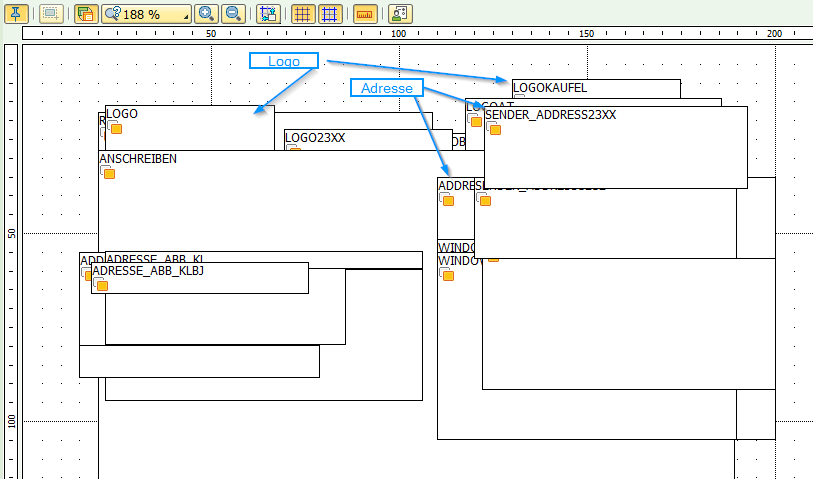
\includegraphics[width=0.65\paperwidth, height=0.4\paperheight]{img/Smartform-Beispiel-1.png}
	\item Unübersichtlichkeit / nicht Wartbar 
\end{itemize}
\newpage
\chapter{Anforderungen}
\label{ch:Anforderungen}



\section{Pflegbarkeit der Inhalte}
	\begin{itemize}
		\item Text in Steuertabellen?
				-> nein weil kein Druckprogramm vorhanden und in der Code-Initialisierung nicht wartbar
		\item Text in Formularfeldern?
	\end{itemize}

\section{Übersetzung}

\subsection{Übersetzung mit Adobe PDF}
				-> Nein weil unübersichtlich und Fehlerbehaftet
\subsection{Steuertabelle für Übersetzung}
				-> Nein da dynamisches Einlesen ohne Druckprogramm schwierig wird
				-> Übersetzten Text in Tabelle ist auch schwierig, da so genannte "Fließfelder" nicht möglich sind.
				Fließfelder sind Abschnitte in einem Text, welche einen dynamischen Inhalt haben aber in den Textfluss mit eingehen. Beispiel: Dieses Dokument wurde am (heutiges Datum) erstellt.
\newpage
\chapter{Umsetzung}

 Nachdem in dem vorhergegangenen Kapitel der aktuelle Stand des Formulars erläutert und die Anforderungen zusammengetragen wurden, wird in dem folgendem Kapitel ein Entwurf erstellt, welcher diese Anforderungen erfüllt. Anschließend wird die Umsetzung der Umstellung auf Adobe \ac{PDF}s beschrieben.


 
\section{Dokument Erstellung}

In den folgenden Abschnitten wird die Erstellung der \ac{LLE} mit Hilfe der Adobe \ac{PDF}s Schritt für Schritt erläutert. Die Abschnitte sind in der selben Reihenfolge gegliedert wie die Durchführung stattgefunden hat.
\subsection{Schnittstelle}

Nachdem in der Transaktion SFP eine Schnittstelle erstellt wurde, werden zunächst die Import-Parameter festgelegt. Die Import Parameter geben an, welche Daten das Druckprogramm an das Formular übergibt. Im Fall der \ac{LLE} sind diese Parameter vom SAP Standard vorgegeben.
Diese Daten beinhalten die Druckparameter, sowie die Informationen, welche den Inhalten des Formulars bestimmen. 

Da die Import Parameter nicht alle benötigten Informationen der \ac{LLE} beinhalten, werden weitere Variablen bei den Globalen Definitionen hinzugefügt. Der Bereich "`Globale Daten"' stellt Variablen zur Verfügung, welche zusätzlich zu den Import Parametern als Datenträger für die Inhalte der \ac{PDF} dienen können. Des Weiteren werden diese Variablen genutzt, um im Laufe der Dokumentenerstellung importierte Daten weiter zu verarbeiten bzw. neue Daten einzulesen.
Die Globalen Definitionen können im Fall der \ac{LLE} aus der alten Smart Form Version übernommen werden, da die selben Variablen Anwendung finden. 

Auf Grund der Tatsache, dass die \ac{LLE} mit einem SAP Standard Druckprogramm erstellt wird, müssen zusätzliche Daten in der Schnittstelle der Adobe \ac{PDF} eingelesen werden. Im Bereich der "`Initialisierung"' wird in der "`Code-Initialisierung"' mit Hilfe von \ac{ABAP}-Code eine Programmlogik erstellt, welche diese Zusatzinformationen von der Datenbank ausliest und in die davor definierten Globalen Variablen schreibt. Hierzu werden Eingabe- und Ausgabe-Parameter definiert. Die Eingabeparameter beinhalten die nötigen Daten, welche in der Code-Initialisierung benutzt werden, um die benötigten Informationen in die Ausgabeparameter zu schreiben. Beispielsweise wird für die \ac{LLE} in der Initialisierung das passende Firmenlogo für die Gesellschaft ausgelesen, welche das Dokument ausstellt. In Abbildung \ref{figCo} ist zu sehen, dass dafür in den Importparametern die \ac{AH} angegeben ist. Die \ac{AH} ist im GTS die eindeutige Einteilung der Gesellschaften und wird deswegen auch im Customizing als Unterscheidungsmerkmal genutzt. Mit Hilfe dieser Information, wird anschließend das zugehörige Firmen Logo ermittelt.

\begin{figure}[ht]
	\centering
	\makebox[\textwidth][c]{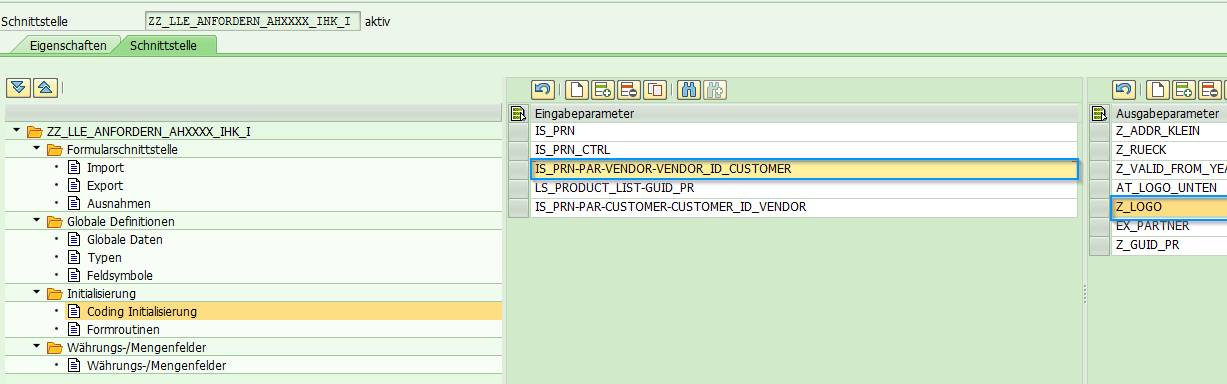
\includegraphics[width=1\textwidth]{img/Init.png}}%		
	\caption{Import- und Export-Parameter in der Code-Initialisierung}
	\label{figCo}
\end{figure}

In diesem Bereich der Schnittstelle ist es ebenfalls möglich, die Daten aus den Importparametern für die Ausgabe aufzubereiten. An vielen Stellen wird in der \ac{LLE} das Jahr abgedruckt, ab dem das Dokument gültig ist. Importiert wird allerdings das gesamte Datum. Um die Verwendung der Jahreszahl zu vereinfachen wird deshalb in der Initialisierung das gewünschte Jahr in eine eigene Variable geschrieben.

Im Fall der \ac{LE} ist die Schnittstelle mit den Globalen Daten und der Code-Initialisierung vollständig. Für andere Formulare gäbe es noch die Möglichkeit, dedizierte Währungsfelder zu definieren. Diese Variablen können den beinhaltenden Wert in jeder gewünschten Währung anzeigen.\footnote{Vgl. \cite{Hauser.2015} S. 138}
Die Schnittstelle kann auch zu späteren Zeitpunkten angepasst werden, falls zusätzliche Variablen benötigt werden oder weitere Logiken in die Initialisierung eingebaut werden müssen.
\FloatBarrier
\subsection{Kontext}

Nach dem Erstellen der Schnittstelle wird das Formular in der Transaktion SFP angelegt. Im Anlageprozess muss unter anderem die zugehörige Schnittstelle angegeben werden. Wie bereits in Kapitel \ref{ch:Aufbau} erläutert, besteht ein Formular im Form Builder aus dem Kontext und dem Layout. Im ersten Teil wird festgelegt, welche der Import- und Globalen-Daten im Layout Bereich für das Dokument zu Verfügung stehen sollen. Zusätzlichen zu diesen Informationen kann die Datenhierarchie bestimmte Bausteine für Texte sowie Adressen beinhalten. Weitere benutzbare Funktionen wie beispielsweise eine Schleifenfunktion dienen dazu, die übertragenen Daten aus der Schnittstelle darzustellen.

Um zu vermeiden, dass Daten und Variablen ungenutzt im Kontext miteinbezogen werden, ist eine gute Vorgehensweise, den Kontext nach Bedarf in mehreren Iterationen mit benötigten Elementen aufzufüllen.


\FloatBarrier
\subsection{Master- und Design-Seiten}
\label{ch:tab}

Den Grundstein des Layouts bilden die Masterseiten. Zunächst wird für jede benötigte Seite eine Masterseite erstellt. In Abbildung \ref{figLLE} ist der Aufbau der \ac{LLE} dargestellt.

\begin{figure}[ht]
	\centering
	\makebox[\textwidth][c]{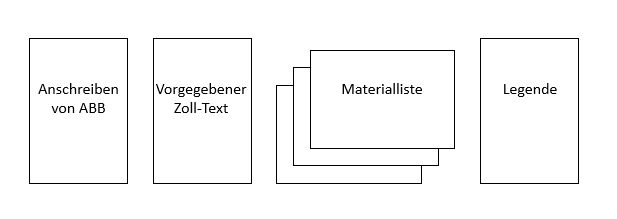
\includegraphics[width=1\textwidth]{img/LLE.png}}%		
	\caption{Aufbau der Lieferantenerklärung}
	\label{figLLE}
	
\end{figure}

Das zweiseitige Anschreiben, der Zoll Text und die Legenden werden im Hochformat und die Materiallisten im Querformat ausgegeben. Die beiden Listen können beliebig lang sein und müssen auf neue Seiten mit dem selben Layout umgebrochen werden.
Die Nummerierung des Dokumentes wird ebenfalls über die Meisterseiten gesteuert. Das Anschreiben soll nicht in die Seitenzahlen miteinbezogen werden, dementsprechend wird in der Objekt Palette dieser Masterseiten eingestellt, dass diese nicht in die Nummerierung aufgenommen werden. Um den Inhaltsbereich der Seiten positionsweise festzulegen, wird auf den Meisterseiten ein Bereich definiert, welcher die Proportionen des Inhaltes eingrenzt. 
  
In der Design Ansicht wird für jede Masterseite auch eine Inhaltsseite eingefügt. Diesen Inhaltsseiten wird in der Objekt Palette bei "`Platzierung"' dem zugehörigen Inhaltsbereich einer Masterseite zugewiesen. Diese Zuweisung führt dazu, dass das Layout der Masterseite und der Inhaltsbereich übernommen wird.

Für die Materiallisten wird in der Objekt-Palette der Inhalt auf "`Textfluss"' umgestellt. Diese Einstellung führt dazu, dass der Inhaltsbereich sich mit dem Inhalt vergrößert, falls mehr Platz nötig sein sollte. Da die Listen über mehrere Seiten abgebildet werden, wird außerdem der Haken in der Palette gesetzt, dass ein Seitenumbruch im Inhalt zugelassen wird.




\FloatBarrier
\section{Einzelne Felder}

Nachdem die Grundstruktur des Formulars mit den Master- und Design-Seiten feststeht wird der Inhalt eingefügt.
Zunächst werden die großen Textfelder für das Anschreiben, sowie die Zolltexte erstellt. Dafür kann die Bibliothek des \ac{ALCD} benutzt werden. Die Felder werden mit Hilfe der Layout-Palette positioniert. Diese Palette dient als Steuerung für alle Layout-Einstellungen eines Elements im \ac{ALCD}. Die Texte werden anschließend in die neu erstellten Felder eingefügt. 

Dynamische Inhalte in Texten können über sogenannte Fließfelder gesteuert werden. Im Fall der \ac{LLE} muss des Öfteren das aktuelle Datum bzw. das Jahr, ab welchem das Dokument gültig ist, in den Text eingefügt werden.
Ein solches Fließfeld wird dementsprechend in den Text eingefügt. Über die Objekt-Palette wird dem Fließfeld eine Datenbindung eingestellt. Diese Bindung verweist auf eine Variable, welche im Kontextbereich definiert wurde. Zum Zeitpunkt des Druckes des Dokumentes wird das Fließfeld durch den Inhalt der verbundenen Variable ersetzt. Der Text um das Feld herum passt sich an die Größe des Inhalts an. In Abbildung \ref{figdt} ist zu sehen, dass Fließfelder im Text durch geschweifte Klammern gekennzeichnet sind.

\begin{figure}[ht]
	\centering
	\makebox[\textwidth][c]{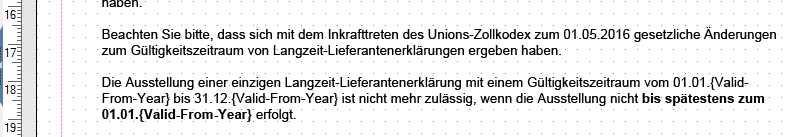
\includegraphics[width=1\textwidth]{img/fliesfeld.png}}%		
	\caption{Fließfelder im Text}
	\label{figdt}
	
\end{figure}



\FloatBarrier
\section{Address Kopf}

Um die vielfachen Adressen in der \ac{LLE} darzustellen gibt es mehrere Möglichkeiten. Die Bibliothek des \ac{ALCD} beinhaltet zwar einen vorkonfigurierten Adressblock, allerdings ist dieser beschränkt auf ein bestimmtes Layout.  Eine andere Möglichkeit ist es, für jeden Adressblock die Felder als Fließfelder anzugeben. Somit besteht keine Beschränkung bezüglich Inhalt und Layout. Alternativ ist es möglich im Kontext Bereich einen sogenannte Adressknoten anzulegen. Diesem Knoten wird eine Adressnummer zugewiesen. Über diese Nummer werden automatisch aus der Datenbank die Adressdaten ausgelesen\footnote{SAP Standard Variante zur Adressenverwaltung}. Diesen Adressknoten kann man im Layout des \ac{ALCD} direkt im Dokument verwenden. Mit Hilfe von Einstellungen, welche man im Kontext Bereich vornehmen kann, wird der Inhalt des Adressblocks gesteuert. Diese Variante eignet sich am besten für standardisierte Adressköpfe.

Im Fall der \ac{LLE} gibt es verschiedenen Informationen welche im Adresskopf angezeigt werden müssen. Ein Block beinhaltet neben den Kontaktdaten zusätzlich noch weitere Informationen zum Dokument, wie beispielsweise der \ac{LLE}-Nummer. Eine anderer Teil des Adresskopfes besteht nur aus dem Standard Name/Straße/Ort Block.
Für die individuellen Adressfelder wird die Methode mit den Fließfeldern angewandt. In Abbildung \ref{figAdr}
ist zu sehen, dass so die Anforderungen am besten umgesetzt werden können.

\begin{figure}[ht]
	\centering
	\makebox[\textwidth][c]{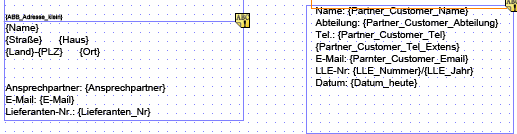
\includegraphics[width=1\textwidth]{img/Adr.png}}%		
	\caption{Adresskopf mit Fließfeldern}
	\label{figAdr}
	
\end{figure}

Für den Standardadresskopf wird die Adressknoten Variante verwendet. Somit wird zunächst im Kontextbereich ein Adressknoten erstellt, welcher die Adressnummer der zugehörigen Adresse beinhaltet. Zusätzlich wird eine Variable angegeben, welche das Absender Land beinhaltet, da davon das Ausgabelayout abhängig ist.

Die Position der Adressköpfe wird festgelegt und ist für jede Gesellschaft gleich. Diese Vereinheitlichung führt zu einer höheren Übersichtlichkeit des Formulars bei zukünftigen Anpassungen. Der Inhalt der Adressen ist ebenfalls ein Zusammenschluss der vielfachen Varianten der früheren Version des Dokumentes.


\FloatBarrier

\section{Tabelle}

Für die Materialliste wird zunächst der Kontext Bereich des Formulars erweitert. Es wird ein Knotenpunkt in Form eines Ordners erstellt, welcher die Elemente der Tabelle beinhalten soll. In diesem Ordner wird anschließend eine Schleife angelegt. Im Fall der \ac{LLE} soll jeder Eintrag der Materialliste im Layout angezeigt werden. Demnach wird in der angelegten Schleife die Materialliste angegeben. Innerhalb der Schleife wird dann eine Zeile dieser Tabelle als Struktur eingetragen. Diese Zeile wird beim erstellen des Formulars mit jedem Eintrag der Materialliste gefüllt. Zusätzlich wird eine Programmknoten in die Schleife eingefügt. Dieser \ac{ABAP}-Code wird ebenfalls bei jedem Durchlauf der Schleife erneut ausgeführt. Diese Programmlogik wird benötigt um Teile der Materialliste für die Darstellung auf dem Formular aufzubereiten.

Nachdem der Kontext Bereich angepasst wurde, wird anschließend die Tabelle im Layout eingebaut. Zunächst wird mit Hilfe des Tabellen-Assistenten des \ac{ALCD} eine Tabelle mit 7 Spalten erstellt. Diese Tabelle wird in einem Teilformular umschlossen. Anschließend wird in der Objekt Palette der Tabelle der Seitenumbruch freigegeben. Des Weiteren wird in der Palette der Kopfzeile eingestellt, dass der Kopf auf jeder umgebrochenen neuen Seite erneut angezeigt werden soll. Um einen Seitenumbruch in Mitten einer Zeile zu vermeiden, wird für die Zeilen ein Umbruch in der Palette nicht erlaubt. 

Nachdem noch weitere Layout Einstellungen, wie Zeilenhintergründe und Größe, vorgenommen wurden, wird anschließend der Inhalt der Tabelle festgelegt. Wie in Abbildung \ref{figTab} zu sehen ist, werden die Daten der Tabelle ebenfalls mit Fließfeldern abgebildet. Aufgrund der vorher festgelegten Schleife wird somit für jeden Eintrag der Materialliste eine neue Zeile ausgegeben.

\begin{figure}[ht]
	\centering
	\makebox[\textwidth][c]{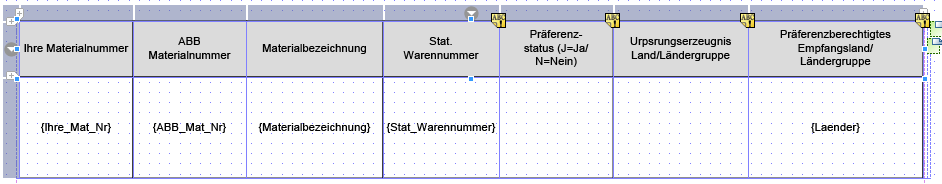
\includegraphics[width=1\textwidth]{img/Tabelle.png}}%		
	\caption{Materialliste mit Fließfeldern}
	\label{figTab}
	
\end{figure}

Um das Layout der Seiten nach einem Umbruch festlegen zu können, wird abschließend in der Objekt-Palette der Seite festgelegt, welche Masterseite für diese Seiten benutzt werden soll. Ansonsten würde die Tabelle auf einer leeren neuen Seite umformatiert weitergeführt werden.

\FloatBarrier
\section{Dynamische Anzeige}
\label{ch:Dyn}

Da die \ac{LLE} von unterschiedlichen Gesellschaften genutzt wird ist es notwendig, dass das Formular sich den jeweiligen Gesellschaften anpasst. Diese Anforderung wird umgesetzt, indem Felder des Formulars, welche im Kontext Bereich definiert wurden, nur unter bestimmten Bedingungen angezeigt werden. Dafür wird ebenfalls im Kontext für die relevanten Felder die Bedingung angelegt, dass sie nur gültig sind wenn eine bestimme \ac{AH} Nummer als Absender eingetragen ist. Anschließend werden im Layout die unterschiedlichen Felder an die bestimmten Positionen gestellt, an welchen der dynamische Inhalte angezeigt werden soll. 

Aufgrund von gesellschaftsspezifischen Anforderungen müssen teilweise Logos an festgelegten Positionen angezeigt werden. Eines dieser festgelegten Logos überdeckt dadurch einen Teil des Adresskopfes, welcher in der alten Version der \ac{LLE} für diese Gesellschaft nicht angezeigt wurde. Um dieses Problem zu lösen wird diesem Teil der Adressen ebenfalls eine Bedingung eingetragen, um die Ausgabe bei dieser Gesellschaft zu unterbinden.  

Die Anzeige der Logos wird mit Hilfe von Grafikelementen umgesetzt, welche im Kontext definiert werden können. Diese Elemente funktionieren in einer ähnlichen Weise wie die Adressfelder. Durch die Zuweisung einer Variablen, die den Namen des Logos beinhaltet, wird das Bild automatisch aus der Datenbank ausgelesen. Diese Methode funktioniert ausschließlich dann, wenn die benötigten Grafiken auf der Datenbank abgespeichert sind.

Zusätzlich zu den bedingten Inhalten muss das Formular in der Lage sein, auf den dynamischen Inhalt reagieren zu können. Im Fall der \ac{LLE} ist ein dynamischer Inhalt die Materiallisten. Da diese Listen eine beliebige Länge erreichen können ist es notwendig, dass die Ausgabe durch automatische Seitenumbrüche trotzdem funktioniert. Wie bereits in Kapitel \ref{ch:tab} beschrieben ist die durch die Textfluss Option gelöst.
Die Seitenzahlen des Formulars müssen ebenfalls dynamisch an den Inhalt angepasst sein.

\FloatBarrier

\section{Ausgabe}

Nach der Fertigstellung des Formulars gilt es, die neue PDF Form im Customizing jeder Gesellschaft zuzuordnen. Nachdem diese Einstellung vorgenommen wurde, kann nun die \ac{LLE} in Form einer PDF ausgegeben werden. Weitere Anpassungen sind nicht nötig.



\newpage
\chapter{Ergebnis}

Ergebnis
\newpage


%	Literaturverzeichnis
\ihead{} % Neue Header-Definition
\printbibliography[title=Literaturverzeichnis]
\cleardoublepage

% Der Anhang beginnt hier - jedes Kapitel wird alphabetisch aufgezählt. (Anhang A, B usw.)
\appendix
\ihead{\appendixname~\thechapter} % Neue Header-Definition

% appendix.tex einziehen
\chapter{Anhang}
\section{Abbildungen}

\begin{figure}[ht]
	\centering
	\makebox[\textwidth][c]{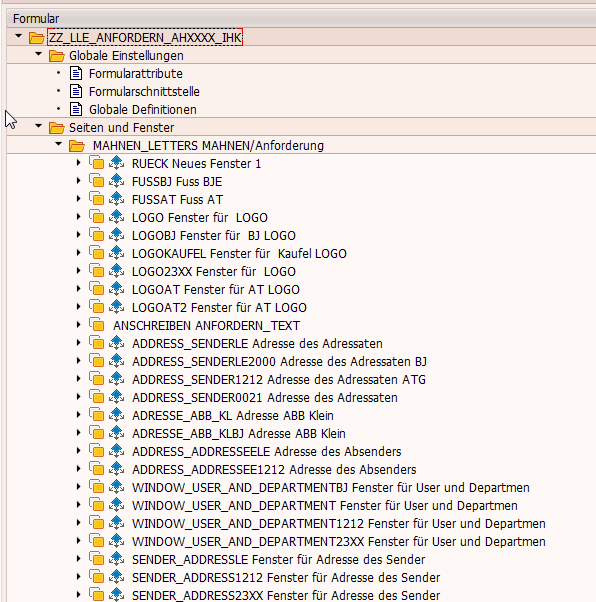
\includegraphics[width=1\textwidth]{img/Smartform_Struktur_1.png}}%		
	\caption{Struktur der \acs{LLE} in Smart Forms}
	\label{AN:Smart1}
\end{figure}

\restoregeometry

\begin{figure}[ht]
	\centering
	\makebox[\textwidth][c]{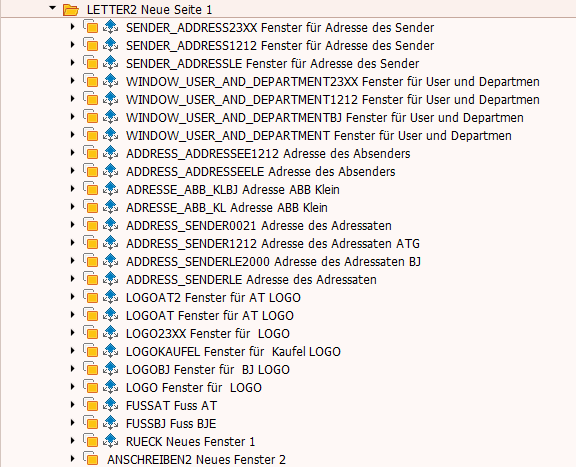
\includegraphics[width=1\textwidth]{img/Smartform_Struktur_2.png}}%		
	\caption{Struktur der \acs{LLE} in Smart Forms}
	\label{AN:Smart2}
\end{figure}

\begin{figure}[ht]
	\centering
	\makebox[\textwidth][c]{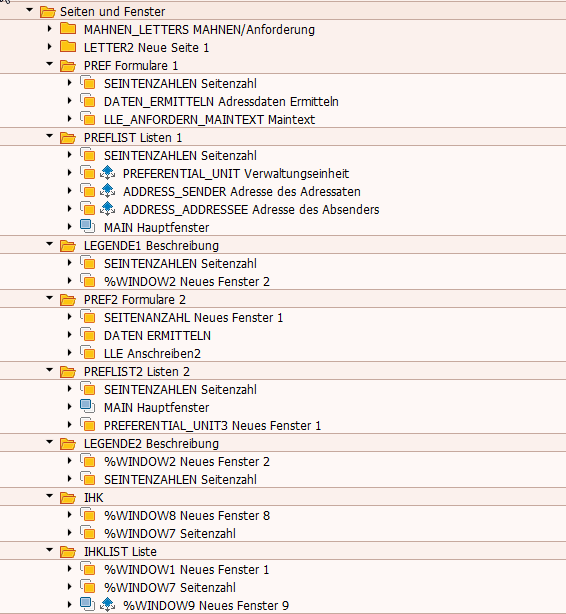
\includegraphics[width=1\textwidth]{img/Smartform_Struktur_3.png}}%		
	\caption{Struktur der \acs{LLE} in Smart Forms}
	\label{AN:Smart3}
\end{figure}

\FloatBarrier

\section {Beispiel Dokumente}

\begin{figure}[ht] \centering{
		
\includegraphics[scale=0.51]{at.pdf}}
	\caption{Anschreiben der \acs{LLE} per Smart Forms für die \acs{AH} 3001}
		\label{AN:lleat}
\end{figure} 

\begin{figure}[ht] \centering{
		
\includegraphics[scale=0.70]{bje.pdf}}
	\caption{Anschreiben der \acs{LLE} per Smart Forms für die \acs{AH} 2000}
	\label{AN:llebj}
\end{figure} 




% Ehrenwörtliche Erklärung ewerkl.tex einziehen
% !TEX root =  master.tex

\clearpage
\chapter*{Ehrenwörtliche Erklärung}

% Wird die folgende Zeile auskommentiert, erscheint die ehrenwörtliche
% Erklärung im Inhaltsverzeichnis.

% \addcontentsline{toc}{chapter}{Ehrenwörtliche Erklärung}
Ich versichere hiermit, dass ich die vorliegende Arbeit
 mit dem Thema: \textit{\DerTitelDerArbeit} selbstständig verfasst und keine anderen als die angegebenen Quellen und
Hilfsmittel benutzt habe. Ich versichere zudem,
dass die eingereichte elektronische Fassung mit der gedruckten Fassung übereinstimmt.

\vspace{3cm}
Ort, Datum \hfill \DerAutorDerArbeit



\end{document}
